\documentclass[../../diss.tex]{subfiles}
\begin{document}

% \chapter{Introduction}
% \label{Chapter:Intro}

Which problems can be solved by computers -- and how?
This question lies at the heart of computer science.
\emph{Theoretical computer science} studies which problems can be solved \emph{in principle}.
To approach this difficult question, we start from the related area of \emph{verification}.
Verification problems consist of checking whether a given system -- usually a program, specified by its source code -- is correct with respect to a certain specification.
Interest in verification is also motivated by its practical importance, given the ubiquity of computers, in particular their usage in applications like aviation where failure may lead to lethal accidents.
The deep link between verification and theoretical computer science comes from the theme of \emph{self-application}:
To understand which problems can be solved by computers, one tries to understand which properties of computers can be decided by other computers.
The principle of self-application has a history reaching back to the beginning of the axiomatization of mathematics and theoretical computer science, demonstrating the usefulness of the approach.
It is used in Russel's paradox~\cite{Russell03}, in the proof of Gödel's incompleteness theorem~\cite{Goedel31}, and in the proof of Turing's famous result that the halting problem is undecidable~\cite{Turing36}.

In fact, Turing's result can be understood as a contribution to the area of verification.
He essentially has shown that it is impossible to algorithmically check the termination of a given (imperative) program.
Similarly, Church's earlier undecidability result~\cite{Church36} for checking the equivalence of $\lambda$-calculus terms can be understood in terms of functional programs: It is not decidable if two given programs have the same runtime behavior.
Finally, Rice's theorem~\cite{Rice53} shows that the problems studied by Church and Turing are not undecidable because of their exceptional hardness.
Rather, these are problems for which the proof of undecidability is not too difficult.
Any other problem in the area of verification is just as undecidable:
A computer cannot decide non-trivial properties of other computer systems in general.

This undecidability conflicts with the practical interest in verification, caused by the need for correct programs in safety-critical applications.
A number of workarounds have risen to fame, including the unit tests and path coverage tests that are the current industry standard~\cite{Beizer90,MyersSB12}.
However, these tests only show the absence of incorrect behavior in certain executions selected by a human.
In order to prove the absence of bugs in \emph{all} executions, researchers in theoretical computer science have developed models that make it easier for humans to prove correctness by hand, like abstract state machines~\cite{Gurevich00,Borger97}, and they have also developed methods for computer-aided verification.
For example, a method based on Hoare logic~\cite{Hoare69} may complete a proof of correctness after certain parts of it, so-called loop invariants, have been specified by a human.

\begin{figure}[t]
    \centering%
    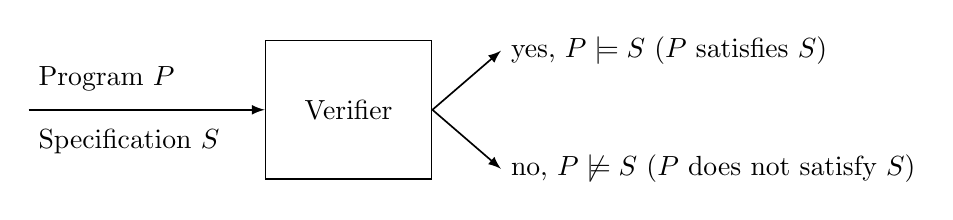
\begin{tikzpicture}[->,>=latex,node distance=7em,semithick]

\node (origin) [coordinate] at (0,0) {};
\node (rect) at (3,0) [minimum width=6em,minimum height=5em, anchor=west,draw] {};
\node (yes) [coordinate] at (6,0.75) {};
\node (no) [coordinate] at (6,-0.75) {};
\path [->,]
    (origin) edge (rect.west)
    (rect.east) edge (yes)
    (rect.east) edge (no)
;

\node at (0,0.4) [anchor=west] {Program $P$};
\node at (0,-0.4) [anchor=west]  {Specification $S$};
\node [right of=yes, node distance=0em, anchor=west] {yes, $P \models S$ ($P$ satisfies $S$)};
\node [right of=no, node distance=0em, anchor=west] {no,  $P \not\models S$ ($P$ does not satisfy $S$)};
\node at (rect) {Verifier};

\end{tikzpicture}
%
    \caption{An ideal verifier.}%
    \label{Figure:IntroVerification}%
\end{figure}

Regardless of the advances in these areas, the fully automatic verification of programs remains the ultimate goal: A computer system that checks all executions of a program for correctness within finite time, without requiring the time investment by or the ingenuity of a human.
% Regardless of the advances in these areas, the fully automatic verification of programs remains the ultimate goal: A computer system that checks all executions of a program for correctness within finite time, neither requiring the time investment nor the ingenuity of a human.
\cref{Figure:IntroVerification} depicts such an ideal verifier.
The undecidability results by Church, Turing, and Rice prove that it cannot exist, but luckily, they leave two loopholes that one can exploit.
The first one is that the results state that verification cannot be solved in general, \ie for all input programs.
The second loophole is that the undecidability results apply to a scenario that is symmetric: Both the input and the solver come from the class of general computer programs.

The first loophole means that it may be possible to construct an algorithm that is able to determine the correctness of \emph{some} input programs in finite time, while it may fail to do so for others.
In fact, many verification problems are semi-decidable, \eg for some verification problem, it may be possible to always find a violation of the specification within finite time if the input program is indeed incorrect.
An algorithm for the problem that can always disprove correctness in finite time while also being able to prove correctness for some programs does not violate the aforementioned undecidability results while potentially being very useful in practice.

The second loophole means that if we assume that we want to solve a verification problem using a general computer, but the input programs come from a restricted class of programs, the undecidability results do not apply.
This has led to various classes of systems, so-called \emph{automata}, being studied in the context of verification.


\paragraph{Automata}

We use automata as a broad term for all kinds of computational devices that have a finite description.
This includes both models for general computers or computer programs, like Turing machines, and weaker models.
If we study verification problems for weaker models, \ie with the assumption that the program that is the input to the verification problem is from a certain class of automata, we can hope for the problem to be decidable.
Automata theory, the subarea of theoretical computer science which studies automata, provides a long list of these models that differ from each other mainly in two ways.
The first is how expressive they are, \ie how close they are to being able to model a real computer.
The second is how amenable they are to automatic verification, \ie which verification problems can be solved algorithmically if we assume the input programs come from that class, and if they can be solved, how efficiently.
As expected, there is a tradeoff between the two aspects:
Instances of a very simple model can be analyzed easily, but they are not very expressive.
Turing machines, a complex type of automata, are able to model any real-world computer program, but the undecidability results apply and automatic verification is impossible.
We will provide more examples for automata models later.

Combined, the two aforementioned loopholes enable the automata-theoretic approach to verification.
Given a verification problem, one constructs an algorithm that works in two steps.
The first step is an \emph{abstraction} step that transforms the input program into an instance of an automata model.
In the second step, one invokes an algorithm for the equivalent verification problem for that class of automata.
The hope is that the output of the algorithm deciding the verification problem for the automaton coincides with the desired answer to the verification problem for the given input program.

\begin{figure}[t]
    \centering%
    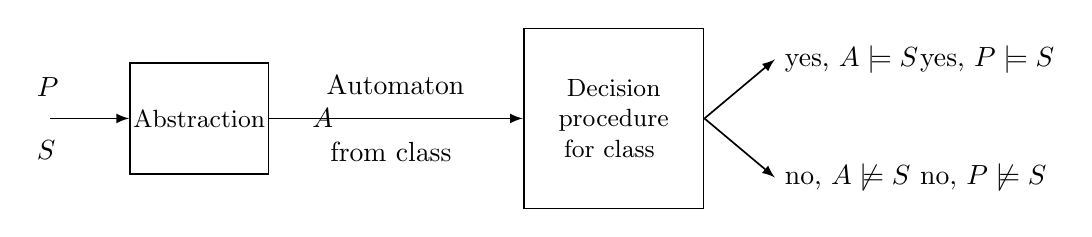
\begin{tikzpicture}[->,>=latex,node distance=7em,semithick]

\node (origin) [coordinate] at (0,0) {};

\node (abstr) at (1,0) [minimum width=5em, minimum height=4em, anchor=west,draw] {};


\node (rect) at (6,0) [minimum width=6.5em,minimum height=6.5em, anchor=west,draw] {};

\node (yes) [coordinate] at (9.2,0.75) {};
\node (no) [coordinate] at (9.2,-0.75) {};
\path [->]
    (origin) edge (abstr.west)
    (abstr.east) edge (rect.west)
    (rect.east) edge (yes)
    (rect.east) edge (no)
;

\node at (-0.3,0.4) [anchor=west] {$P$};
\node at (-0.3,-0.4) [anchor=west] {$S$};

\node at (3.2,0) [anchor=west, align=center, text width=6em] {Automaton $A$ \newline from class $\calC$};

\node (yes2) [right of=yes, node distance=0em, anchor=west] {yes, $A \models S$};
\node (no2) [right of=no, node distance=0em, anchor=west] {no, $A \not\models S$};

\node [align=center, font=\small] at (abstr) {Abstraction};
\node [align=center, text width=5em,font=\small] at (rect) {Decision procedure for class $\calC$};

\node (yes3) at (10.8,0.75) [anchor=west] {$\implies$ yes, $P \models S$};
\node (no3) at (10.8,-0.75) [anchor=west]  {$\implies$  no, $P \not\models S$};

\end{tikzpicture}

    \caption{An ideal verifier using the automata-theoretic approach.
    % The notation is as in \cref{Figure:IntroVerification}.
    % Note that such a general algorithm cannot be designed in practice: If class $\calC$ is Turing-powerful, non-trivial properties of automata are undecidable and the required decision procedure does not exist.
    % If the automata in class $\calC$ are weaker, the answer provided by the decision procedure ($A \models S$ \resp $A \not\models S$) does not have to coincide with the answer to the verification problem ($P \models S$ \resp $P \not\models S$).
    }%
    \label{Figure:IntroAutomata}%
\end{figure}

A schematic ideal verifier using this automata-theoretic approach is depicted in \cref{Figure:IntroAutomata}.
Unfortunately, just like the more general ideal verifier, it cannot exist.
Assume we choose a class of automata that is expressive enough to capture the behavior of real computer programs as the target of the abstraction.
Then the decision problem for this class of automata that corresponds to the undecidable verification problem that we want to solve is also undecidable.
If we choose a strictly weaker class, the corresponding decision problem might become decidable.
However, in that case, the abstraction will lead to a loss of information.
We cannot guarantee that the answer to the decision problem, \ie whether the automaton satisfies the specification, is equal to the answer to the verification problem, \ie whether the program \nb{satisfies the specification}.

One way to circumvent this problem is to choose the abstraction carefully.
This includes choosing the right class of automata as the target for the abstraction.
We will come back to this aspect at the end of this section when we mention various models of automata and their strengths and weaknesses.
For now, we focus on a more general approach that works for various classes of automata.
The idea is to choose the abstraction so that it either underapproximates or overapproximates the given program.
These are ways to abstract a program into an automaton from a restricted class, thus avoiding undecidability, while still retaining some information.
%about the initial program.

An \emph{underapproximation} yields an automaton so that any execution of the automaton represents a valid execution of the program, but not every execution of the program is necessarily reflected in the behavior of the automaton.
Consequently, an execution of the automaton violating the specification is also an execution of the program violating it.
In summary, we obtain that if the automaton violates the specification, so does the program.
If the automaton satisfies the specification, we do not know whether the initial program is indeed correct or whether it was incorrect, but the abstraction has led to losing the violating executions.
Hence, underapproximations are useful for finding bugs, but a priori they are not suitable \nb{for proving correctness}.

An \emph{overapproximation} leads to an automaton with a larger set of possible executions:
Any execution of the program is represented by an execution of the automaton, but the automaton may have additional \emph{spurious executions}.
If the automaton is then shown to be correct, all its executions -- including all executions of the original program -- satisfy the specification.
If the automaton is incorrect, we do not know whether this comes from the program being incorrect or whether it is caused by a spurious execution introduced by the abstraction.
Hence, overapproximations are suitable for proving correctness, but in order to handle incorrect input programs, we would need some way to deal with spurious violations of the specification.
Both \nb{concepts~--~underapproximations} and \nb{overapproximations~--~are} depicted in \cref{Figure:IntroAutomataApproximation}.
In the rest of this chapter, we will focus on examples using overapproximations.

\begin{figure}[t]
    {%
        \centering
        \subcaptionbox{Using overapproximation.\label{Figure:IntroAutomataApproximationOver}}[0.49\textwidth][c]
        {%
            \scalebox{0.75}
            {%
                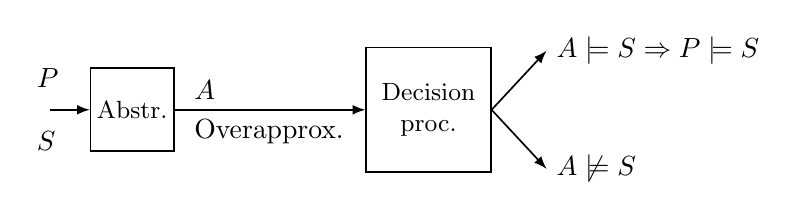
\begin{tikzpicture}[->,>=latex,node distance=7em,semithick]

\node (origin) [coordinate] at (0,0) {};

\node (abstr) at (0.5,0) [minimum width=3em, minimum height=3em, anchor=west,draw] {};


\node (rect) at (4,0) [minimum width=4.5em,minimum height=4.5em, anchor=west,draw] {};

\node (yes) [coordinate] at (6.3,0.75) {};
\node (no) [coordinate] at (6.3,-0.75) {};
\path [->]
    (origin) edge (abstr.west)
    (abstr.east) edge (rect.west)
    (rect.east) edge (yes)
    (rect.east) edge (no)
;

\node at (-0.3,0.4) [anchor=west] {$P$};
\node at (-0.3,-0.4) [anchor=west] {$S$};

\node at (1.7,0) [anchor=south west] {$A$};
\node at (1.7,0) [anchor=north west] {Overapprox.};


\node (yes2) [right of=yes, node distance=0em, anchor=west] {$A \models S \Rightarrow P \models S$};
\node (no2) [right of=no, node distance=0em, anchor=west] {$A \not\models S$};

\node [align=center, font=\small] at (abstr) {Abstr.};
\node [align=center, text width=5em,font=\small] at (rect) {Decision proc.};

\end{tikzpicture}

            }
        }
    }
    {%
        \centering
        \subcaptionbox{Using underapproximation.\label{Figure:IntroAutomataApproximationUnder}}[0.49\textwidth][c]
        {%
            \scalebox{0.75}
            {%
                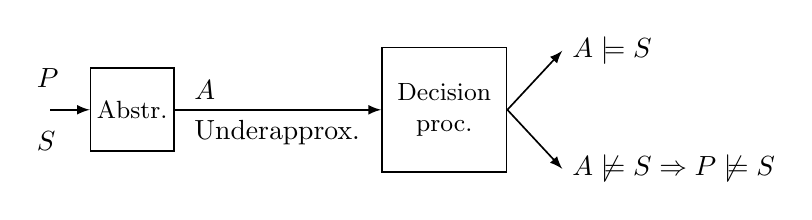
\begin{tikzpicture}[->,>=latex,node distance=7em,semithick]

\node (origin) [coordinate] at (0,0) {};

\node (abstr) at (0.5,0) [minimum width=3em, minimum height=3em, anchor=west,draw] {};


\node (rect) at (4.2,0) [minimum width=4.5em,minimum height=4.5em, anchor=west,draw] {};

\node (yes) [coordinate] at (6.5,0.75) {};
\node (no) [coordinate] at (6.5,-0.75) {};
\path [->]
    (origin) edge (abstr.west)
    (abstr.east) edge (rect.west)
    (rect.east) edge (yes)
    (rect.east) edge (no)
;

\node at (-0.3,0.4) [anchor=west] {$P$};
\node at (-0.3,-0.4) [anchor=west] {$S$};

\node at (1.7,0) [anchor=south west] {$A$};
\node at (1.7,0) [anchor=north west] {Underapprox.};


\node (yes2) [right of=yes, node distance=0em, anchor=west] {$A \models S$};
\node (no2) [right of=no, node distance=0em, anchor=west] {$A \not\models S \Rightarrow P \not\models S $};

\node [align=center, font=\small] at (abstr) {Abstr.};
\node [align=center, text width=5em,font=\small] at (rect) {Decision proc.};

\end{tikzpicture}

            }
        }
    }
    \caption{%
        Verifiers using the automata-theoretic approach as in \cref{Figure:IntroAutomata}, but the abstraction approximates the behavior of the input program.
        We may avoid undecidability, but only in one of the two cases, the answer provided by the decision procedure has mandatory implications for the correctness of the input program.
    }%
    \label{Figure:IntroAutomataApproximation}
\end{figure}

One way to obtain an overapproximation of a program is by using a control flow abstraction.
This means we abstract a program into an automaton that just models the control flow, while we discard the data values.
Conditional branching in the program that jumps to one of several branches depending on a data value is replaced by the nondeterministic choice among these branches in the automaton.
Consequently, even if the input program was deterministic, the result of the control-flow abstraction is typically a nondeterministic automaton whose behavior is an overapproximation of the program.
%
The overapproximation can be made more precise using \emph{predicate abstraction}~\cite{GrafS97}.
We assume that we have a finite collection of predicates, functions that map the state space of the program (including the data values) to Boolean values.
In addition to the control flow of the program, the automaton that is the result of applying predicate abstraction also keeps track of the values of these predicates.
We can resolve conditional branching deterministically whenever the description of the data values provided by the predicates is sufficiently precise.
\nb{Otherwise, we still rely on nondeterminism}.\footnote{%
    For example, consider a program storing an integer $n$.
    Instead of storing $n$, a predicate abstraction may just store the parity of $n$.
    When the program branches depending on whether $n$ is even, we can resolve this choice.
    When it branches depending on whether $n$ equals $0$, we have to use nondeterminism.
    Similarly, when an instruction increments $n$ by one, we can update the state of automaton deterministically because an increment will flip the parity of $n$.
    When an instruction halves $n$, we have to use nondeterminism as we do not know the resulting parity.
}
The result is still an overapproximation, but depending on the choice of the predicates, it can be much more precise than a simple control flow abstraction.

The concept of approximations gives us a template for the construction of verification procedures that are useful, although not very sophisticated.
(We will discuss more involved concepts that can deal with \eg the shortcomings of overapproximations later.)
In order to instantiate this template, one needs abstractions and decision procedures for automata models.
Practical research in verification has come up with a wide selection of abstractions that transform programs into instances of various automata models.
While we mention a few of them below, abstractions are not the focus of this thesis.

The goal of this thesis is to enrich the toolkit of automata theory by providing procedures that solve decision problems related to automata with optimal resource consumption.
We observe that in order to be useful in practice, a verification procedure that uses automata often needs \emph{to produce and use certificates} and to \emph{interact with the environment}.
Hence, the decision procedures that we contribute should take these aspects into account.
In the rest of this section, we will explain what we mean by certificates and the environment.
We will then give an introductory example, demonstrating the usefulness of \nb{these concepts}.


\paragraph{Certificates}

Before discussing why certificates are useful in the context of the automata-theoretic approach to verification, we will give a general definition.
Assume we have an instance of a decision problem and the information whether it is a yes- or a no-instance.
A certificate is additional information that proves that the Boolean yes/no answer is indeed correct.
Typically, it is easier to verify the answer using the certificate than to compute the answer without prior knowledge.

An easy example is intersection-emptiness problems.
Assume we are given two (representations of) sets.
It is usually easier to verify that a given element is contained in both sets than to compute that the two sets have a non-empty intersection.
Hence, an element of the intersection can serve as a certificate for the non-emptiness of the intersection of two sets.
Verification problems can often be seen as intersection-emptiness problems:
A program represents a set of possible executions while a specification gives rise to a set of executions that violate the specification.
If the two sets are disjoint, all possible executions are valid and the program is correct.
If the two sets have a non-empty intersection, the program is incorrect.
An element of the intersection as a certificate for non-emptiness is an execution of the program that violates the specification.
Hence, it is indeed a certificate for the incorrectness of the program.
Producing certificates in the case of an empty intersection \resp a program that is correct is a more involved problem that we will discuss in the next section of this chapter, \cref{Section:IntroSeparability}.

It is noteworthy that the modern definition of the important complexity class $\NPTIME$~\cite{Cook00} also uses certificates.
Traditionally, $\NPTIME$ has been defined as the problems solvable by nondeterministic Turing machines (NTMs) in polynomial time.
NTMs are a model that is often perceived to be hard to understand, in particular because NTMs cannot be implemented in practice.
To circumvent this problem, $\NPTIME$ can equivalently be defined as the class of decision problems such that each yes-instance has a certificate that allows a deterministic algorithm to verify that it is indeed a yes-instance (with the constraint that the size of the certificate and the running time of the verifier are polynomial).

There are multiple reasons for being interested in algorithms that do not only compute a yes/no answer for a decision problem that they solve, but also a certificate.
Firstly, it makes the algorithms accountable:
Instead of blindly trusting the result produced by a procedure, the certificate can be used to check its correctness.
This makes it easier to develop advanced and highly optimized algorithms that are correct by using a well-understood and less-optimized procedure to check the certificates during the development process.
For example, in the SAT competition, a competition in which state-of-the-art algorithms for the satisfiability problem of propositional logic are benchmarked, the algorithms are required to provide certificates both for yes- and for no-instances~\cite{Satcomp18}.

Secondly, there are cases in which it is not the Boolean answer to the decision problem that is relevant in practice, but the certificate for that answer.
This is true in particular for verification problems:
If the answer to a verification problem is negative and the program is incorrect, the developers of the program will most likely require a violating execution to be able to find, understand, and resolve a bug in the program.
In the last section of this chapter, we will briefly discuss decision problems related to synthesis for which a certificate for the answer, a so-called \emph{strategy}, is needed in order to actually perform the synthesis task.

Verification procedures that use the automata-theoretic approach may invoke a decision procedure not once, but multiple times.
For example, each invocation may correspond to a different part of the system that should be verified.
The first call produces a certificate and subsequent calls will take the certificates produced by earlier calls as additional inputs.
We will discuss compositional verification as an example for this concept in detail later.
Alternatively, a procedure may work with a sequence of refinements of the abstraction of the system, calling the decision procedure once for each refinement.
To refine an abstraction in that sequence in order to obtain the next one, one calls the decision procedure and then uses the resulting certificate.
We briefly discuss the CEGAR loop as an example.

\emph{Counter-example guided abstraction refinement (CEGAR)}~\cite{ClarkeGJLV00} is a technique that was first developed in the context of \emph{abstract interpretation}.
Abstract interpretation~\cite{CousotC77} is an approach to verification that is in a certain sense the antithesis to the automata-theoretic approach.
The automata-theoretic approach takes the input program, abstracts it, and then computes precise information about the abstraction.
Abstract interpretation takes the unmodified program and computes imprecise or abstract information about it, in the hope that this information is sufficient to settle the answer to the verification problem.
In spite of this contrast, many techniques can be brought from one world to the other.
For example, the CEGAR approach was brought to the world of automata theory by Podelski and his coauthors, see \eg \cite{HeizmannHP10}.
We have previously mentioned that an overapproximation of a program is useful for verification in the sense that if the overapproximation is correct, then so is the initial program.
If the overapproximation is incorrect, we will have to determine whether this is due to an execution of the initial program that violates the specification, or just due to a spurious execution introduced by the overapproximation.
The CEGAR approach consists of constructing an initial overapproximation, and then executing the following steps in a loop:
We verify the current overapproximation by calling an automata-theoretic decision procedure.
If the overapproximation is correct, then so is the program and the procedure terminates.
Otherwise, we assume that the decision procedure yields an incorrect execution as the certificate.
We check whether the violating execution is indeed an execution of the given program.
In contrast to the verification problem, this is a decidable question.
If the violating execution is a real execution of the program, the program is incorrect and the procedure terminates.
Otherwise, the violating execution is a spurious counterexample, and we can obtain a proof for its spuriousness as a second certificate.
We then use this proof as a guide to construct the description of a set of spurious counterexamples that includes the one that we obtained earlier.
We construct a new overapproximation whose set of possible executions is the old set of possible executions minus this set, then restart the loop.

Discussing the details of the procedure, \eg how we check whether an execution is spurious and how the refinement works in detail, is beyond our scope.
If the basic CEGAR principle outlined here is combined with some implementation tricks, one ends up with a procedure that has been shown to perform well in practice~\cite{HeizmannCDGNMSS17}.
The loop is not guaranteed to terminate, meaning that the CEGAR approach does not solve the verification problem within finite time in all cases and hence its existence does not contradict the undecidability results.
Even if the program is correct, we may not be able to find an overapproximation that is precise enough to prove correctness within finite time.
Similarly, even an incorrect program that actually has a violating execution may still cause us to consider spurious executions in the loop ad~infinitum.
However, for many programs of practical interest, the procedure will within finite time either prove that the program is correct by finding a suitable overapproximation or prove incorrectness by finding a violating execution.
Certificates are crucial in two steps of the loop in order to deal with spurious counterexamples:
We need a certificate to decide whether a violation that we have found is spurious, and we need a certificate for the refinement of the approximation.
Hence, certificates are absolutely essential to make the CEGAR approach work.

\paragraph{The environment}

When we apply an automata-theoretic decision procedure to an abstraction of a system, there is a part of the system that is not reflected in the automaton because it has been lost during the abstraction.
We call this part of the system the \emph{environment}.
It is \emph{hostile} to the verification process because it is the essence of what may prevent the result of the decision procedure from coinciding with the desired answer to the original verification problem.
In order to succeed at verification, an algorithm has to interact with the hostile environment at some point.
Only if we make sure that every possible behavior of the environment is taken into account, we can guarantee that the output of the decision procedure is correct.

In an algorithm that is based on overapproximation, the environment corresponds to the set of spurious executions.
These are the executions that are present in the automaton but not in the initial program.
If the abstraction that is obtained by overapproximating is correct, one can deduce the correctness of the program; the environment has been taken care of by the overapproximation.
But if the abstraction is incorrect, interacting with the environment is necessary in order to have a chance at completing the verification task.
In the aforementioned CEGAR approach, if the algorithm finds that the current overapproximation violates the specification, it queries the environment in order to check whether the violating execution is spurious.
If it is, we also obtain from the environment a proof of spuriousness that is then used for refinement.
Only by using the environment, we can obtain a powerful tool that can deal with real programs even if the initial overapproximation is not correct.

The initial system that the verification procedure is starting with is usually not living in a vacuum, but also in what is often called an environment.
For example, a program may accept user inputs or it may communicate with a reactive system like a database server.
These external dependencies are typically not fully specified in a description of the system.
Our notion of environment may seem to be in conflict with this type of environment.
However, we argue in the following that the two notions of environment are essentially the same.

Firstly, the two types of environments play the same role.
In both cases, we are interested in the correctness of a system, but our algorithm has to work with an abstract description of the system that is missing some parts.
It does not matter whether the description is incomplete because we have applied an abstraction to a more comprehensive model of the system, or whether the description is missing some external dependencies that were never explicitly \nb{modeled to begin with}.

Secondly, the two types of environments usually manifest themselves in the same way in the abstraction.
Hence, they can also be dealt with in the same way.
For example, it is common to model external dependencies using nondeterministic branching:
A program location at which the program queries a database server can be seen a nondeterministic choice between various transitions, one for each possible result.
Nondeterminism also comes into play when we apply an abstraction.
As we have explained earlier, an abstraction that removes a data value means that conditional branching in the program that depends on this data value has to be turned into nondeterministic branching in the automaton.
In both cases, the abstraction overapproximates the behavior of the original program.
This imprecision is handled by seeing the nondeterminism as hostile to the verification task.
A nondeterministic system is usually only considered to be correct if all of its executions that may result from resolving the nondeterminism at runtime are correct.
When we find a violating execution, we may interact with the environment to find out whether the execution is spurious.
If the nondeterminism comes from an external dependency like a database server, we might check a specification of the database server to find out if the behavior in the spurious execution is actually possible.
If the nondeterminism comes from the abstraction that we had applied earlier, we might check whether the execution is a valid execution of the original program, like in the CEGAR loop.
In the rest of this thesis, we will not conceptually distinguish the two types of environment.

We give some additional examples on how a verification algorithm may take the environment into account.
Each of these examples corresponds to one of the three main topics that this thesis is concerned with.
In each example, the way in which the environment is specified and hence also the way in which it is interacted with is different.

The first example is the case of a system with which we interact through unreliable communication.
We have a description of the system, but what we are actually interested in is its visible behavior.
Hence, we may see the unreliability of the communication channel as an environment that has to be taken into account.
We do not have a precise description of the environment and will assume that it is either lossy, \ie it only removes messages from the communication channel, or gainy, \ie it only adds messages.
This allows us to compute a description of the behavior of the overall system (\ie after taking the communication into account) that is larger but conceptually simpler than the description we started with.
We discuss the details in the second section of this chapter, \cref{Section:IntroClosures}, and the corresponding theory in \cref{Part:Closures}.~of this thesis.

In our second example, we consider games, \ie systems with two types of nondeterminism.
One type of nondeterminism is uncontrollable \emph{demonic} nondeterminism which corresponds to the environment and is hostile to the verification task.
Additionally, there is controllable \emph{angelic} nondeterminism.
The latter can be instantiated at runtime to react to the nondeterministic choices of the environment in order to obtain an execution satisfying a specification.
The goal is to find an instantiation that always reacts correctly.
This setting appears in some verification tasks, \eg when both the system and the specification are modeled as nondeterministic automata.
Such a system is correct if for each of its branches, there is a matching branch of the specification.
Additionally, two types of nondeterminism are needed to model program synthesis.
We discuss the details in the third section of this chapter, \cref{Section:IntroGames}, and the corresponding theory in \cref{Part:Games}.~of this thesis.

Our final example is concerned with a compositional approach to the verification of concurrent systems.
The goal is to verify the system component-wise.
When focusing on a single component, the rest of the components become an environment that has to be taken into account.
We explain the details in the following.

\paragraph{Compositional verification}

We consider concurrent systems, systems that consist of multiple components that run concurrently and may communicate with each other during runtime.
The verification of such systems is one of the most challenging tasks in the area of verification.
At the same time, the ubiquity of \eg distributed systems means that this task is of the utmost importance.

For the sake of simplicity, we will in the following consider a concurrent system whose components are given as finite(-state) automata.
Finite automata are among the simplest and most restricted types of automata.
A finite automaton consists of a list of finitely many states and a list of the transitions between these states.
At each point during runtime, the automaton is in a specific state.
Other than that, it has no storage that it can manipulate.
With this set of features, a finite automaton can model a program that only uses bounded storage by encoding the stored data as part of the state.
Finite automata support neither recursion nor concurrency.
The advantage of using such a simple model is that the undecidability results do not apply.
For input programs modeled by finite automata, virtually all verification problems are decidable.

While a single finite automaton is simple, a concurrent system whose components are finite automata is not.
Just as other problems in the area of verification of concurrent systems, verifying such a system suffers from the so-called \emph{state explosion problem}.
It would be possible to construct a single finite automaton as a representation for the whole system.
However, since finite automata lack inherent support for concurrency, this leads to an automaton with a huge state space.
Each global state of that automaton is a combination of local states, one for each component, and the global state space is the set of all such combinations.
Assume we add components to the system or enlarge existing ones.
The effect on the size of its description, given as a collection of automata, is additive.
The size of the global state space, however, grows multiplicatively.
Any verification procedure that explicitly explores this global state space usually has a worst-case running time that is exponential in the number of components.

Results in computational complexity theory have led us to believe that it is highly unlikely that this worst-case lower bound can be improved.
In particular, algorithms that do not construct a single finite automaton as a representation of the system, but instead use a model that has inherent support for concurrency like Petri nets, are not any more efficient.
This brings us back to the first loophole that we considered when we wanted to solve undecidable verification problems.
An undecidable problem cannot be solved in full generality, but a procedure may be able to determine the status of some instances within finite time.
Similarly, a problem with a high computational complexity cannot be solved efficiently in the worst case.
However, an algorithm may be able to deal with a large class of inputs that are relevant in practice quickly.
This hope is fueled by advances with respect to similar problems.
For example, satisfiability checking for propositional logic is strongly believed to be impossible with less than exponential time consumption in general.
Nevertheless, there are state-of-the-art tools that can solve instances of practical interest with millions of variables within minutes, see \eg~\cite{LiFLMLL18}.

Several approaches that try to enable efficient verification procedures for concurrent systems are collectively referred to as \emph{compositional verification}~\cite{OwickiG76,Lamport77,MisraC81,Pnueli84}.
They all try to verify each component of a concurrent system on its own, without ever fully exploring the global state space.
If this succeeds, the running time should scale polynomially with the size of the description of the system (including the number of components), instead of exponentially.
Under the presence of some form of communication between the components, however, it is typically impossible to simply consider each component individually.

When we focus on a single component of a concurrent system, the rest of the components turn into an environment.
The effect of the environment on that component usually cannot be disregarded, it has to be taken into account.
In order to avoid the aforementioned state explosion problem, we do not want to explicitly construct a description of the environment.
The hope is that an abstraction of the environment is sufficient to capture the interference caused by it with respect to the verification of the single component that we consider.
When we verify that component, the abstraction is a specification for the behavior of the hostile environment that we can rely on.
However, this results in an additional proof obligation: We have to establish that the environment indeed satisfies its specification.

We argue that the specification of the environment plays the role of a certificate.
If the system at hand consists of two components, we start by focusing on one component.
The goal is to establish a specification that is satisfied by any system containing that component, independent of the interference caused by the other component.
Then, one shows that the whole system is correct by considering the other component.
In order to deal with communication between components, we rely on the specification that has already been established.
For a system with multiple components, one can use an iterative approach.
One considers the components one by one, often starting with the component that is influenced the least by the others.
The algorithm produces a sequence of certificates in the form of specifications for parts of the system until it is finally able to prove the desired property of the whole system.

There is a clear trade-off between the size of the abstraction and the ease of using it to establish correctness.
A precise abstraction resembles the system more closely, which can make it easier to both establish its correctness and to use it to complete the verification of the system.
However, the size heavily impacts the running time of the verification procedure.
In general, there is no guarantee that there is an abstraction of a component that is precise enough to prove correctness while having a substantially smaller description.
Hence, the existing approaches for compositional verification do not contradict the belief that the efficient verification of concurrent systems is impossible in general.
However, the method has been shown to work well in practice.
On the theoretical side, when the components are finite automata, there are algorithms that can find the smallest abstraction of a component that is sufficient to prove correctness based on Angluin's $\text{L}^*$ algorithm~\cite{Angluin87,PasareanuGBCB08}.
When the components are modeled as automata from a less restrictive class, the problem becomes more involved.
We will discuss the details in the next section of this chapter, \cref{Section:IntroSeparability}.

\paragraph{Automata theory}

We conclude this section by coming back to the area of automata theory.
We name some classes of automata and explain their strengths and weaknesses.
This will also explain how an automata model that is suitable as the target of the abstraction in the automata-theoretic approach to verification can be chosen.

We have already mentioned that there are types of automata that are able to model the behavior of a general program, with Turing machines being the most important example.
One believes that these \emph{Turing-complete} models are at the frontier of computability: Each automaton from such a model can be simulated by a real computer, and every algorithm that can be implemented in the physical word, \eg in the form of a computer program, can be modeled as such an automaton.
Unfortunately, each of these models suffers from the undecidability results mentioned at the beginning of this section.
This means that every verification problem in which the goal is deciding a non-trivial property of the behavior of an automaton from a Turing-complete class is undecidable and hence cannot be solved algorithmically in full generality.

We have already briefly discussed finite automata.
This model is very restricted and hence unable to model most real computer programs.
At the same time, virtually all verification problems which take finite automata as inputs are decidable.
Between finite automata and Turing machines, there is a whole hierarchy of models that are more expressive than finite automata while still allowing for some verification problems to be decidable.
We mostly focus on two branches of this hierarchy in the rest of the thesis:
Context-free models like pushdown automata and their extended and restricted variants, and Petri nets and related models.

Pushdown automata are essentially finite automata that maintain a stack to store information during runtime.
To avoid Turing-completeness, this stack can only be accessed in a LIFO (last in, first out) manner.
It is well-understood that pushdown automata are suitable to model programs with recursion by using the stack as a call-stack.
However, pushdown automata cannot model unbounded storage and they have no inherent support for concurrency.
The stack makes them suitable to model the \emph{control flow} of programs in many classical imperative programming languages, \eg C~\cite{C90}, while lacking support for modern features like generics and templates~\cite{Alexandrescu01} and higher-order functions~\cite{Haskell03}.

For pushdown automata, many verification problems like safety, \ie whether a certain error state can be avoided, or liveness, \ie whether a certain good state can be reached indefinitely often, are decidable.
However, some problems that are decidable for finite automata are undecidable for pushdown automata.
For example, it is not decidable whether two pushdown automata can be synchronized in a way such that an error state is reached in both automata.
This corresponds to the fact that pushdown automata cannot deal with concurrency; the combination of two pushdown automata, or alternatively, a pushdown automaton that maintains two stacks, is a Turing-complete model.

In contrast to pushdown automata, Petri nets can deal with concurrency but not with recursion (and neither of the two models can deal with unbounded storage).
A Petri net is essentially a finite automaton in which a potentially unbounded number of threads run simultaneously.
These threads can spawn, terminate, and synchronize during runtime.
Similar to pushdown automata, basic verification problems like safety verification are decidable for Petri nets.
Unlike pushdown automata however, for which safety verification can be done in polynomial time, \emph{coverability}, the algorithmic problem for Petri nets corresponding to safety verification, is much more expensive and needs at least exponential time in general.\footnote{%
In fact the problem is $\EXPSPACE$-complete~\cite{Lipton76}, meaning that solving it in full generality needs at least exponential space in the worst case.
If the commonly held beliefs about the relations between various complexity classes are true ($\EXPSPACE \neq \EXPTIME$), this means an algorithm solving it will need at least super-exponential time.%
}%
% Note that combining the features of both models leads to a model for which the decidability of reachability is unknown, see \eg \cite{Lazic13}.

At the beginning of this section, we have argued that the ultimate goal is to design a verification algorithm that works without human input.
The automata-theoretic approach seems to miss that goal, since it appears that we have to choose an automata model as the target of the abstraction by hand.
However, as we just have discussed, each class of automata has a general set of strengths and weaknesses, \eg Petri nets are useful to model concurrency.
This allows us to pick an automata model for a verification task based on the type of program and the type of specification, without actually looking at the details of the implementation.
It also means that a verification tool using the automata-theoretic approach that has been developed with a specific program in mind is typically also useful for a wide class of similar programs.
If the chosen automata model is not suitable to model certain features of the original program (\eg neither Petri nets nor pushdown automata can deal with unbounded storage), using an iterative approach like the CEGAR loop may help to alleviate the problem.

In addition to the automata-theoretic approach to verification, there is another noteworthy link between automata theory and verification.
The verification problems for various automata are important examples of problems that are complete for certain classes of computational complexity.
This essentially means that a certain type of automaton with unrestricted resource consumption typically corresponds to an unrestricted program with a certain bounded resource consumption.
For example, whether a pushdown automaton reaches a certain error state can be decided in polynomial time.
In turn, any Turing-machine that has a polynomially bounded time consumption can be turned into a pushdown automaton so that the Turing-machine can reach an error state if and only if the pushdown automaton can.
When we introduce a decision problem that is based on automata in the rest of thesis, we will generally also provide a lower bound for the computational complexity of solving that problem.
When we propose an algorithm solving the problem, we will analyze its resource consumption and determine whether it matches the lower bound.

\paragraph{The language-theoretic approach}

Automata theory is closely connected to taking a \emph{language-theoretic approach} to verification.
The basic idea is to associate to a program or system a finite set of atomic actions that the program may execute.
An execution of the system corresponds to a sequence of such actions, and the system itself gives rise to a set of sequences, one for each possible execution.
In the following, we will call the actions \emph{letters}, the set of possible actions an \emph{alphabet}, the sequences of actions \emph{words}, and sets of sequences \emph{languages}.
How we translate actions into letters depends on the verification task at hand.
For example, letters may correspond to assembly commands, packages sent over a network, or read and write accesses to memory locations.

In the same way that a program gives rise to a language, a specification defines a language of legal executions and its complement, the language of illegal executions.
Verifying a program typically amounts to checking an inclusion: The set of possible executions should be a subset of the set of legal executions.
Equivalently, the intersection between the possible and the illegal executions should be empty.

The crucial advantage provided by the language-theoretic approach is a layer of abstraction on top of the internal workings of a system.
For example, it allows us to consider specifications that are independent of the internal design of a system, \eg the reachability of a special error state.
Instead, the specification talks just about the visible behavior of the system.
This allows us to specify the behavior that we want to consider illegal and then verify that it does not occur, without relying on the implementation of the error handling inside the system being correct.

In the following, we will use the operator $\lang{-}$ to associate a language to a system or specification.
The verification problem for a system $A$ and a specification $\varphi$ is typically equivalent to the question of whether the inclusion $\lang{A} \subseteq \lang{\varphi}$ holds.
We assume that there is a common alphabet $\Sigma$ so that both $\lang{A}$ and $\lang{\varphi}$ are subsets of $\Sigma^*$, the set of all finite words formed using letters from $\Sigma$.
Note that in principle, it is possible to also consider languages of infinite words, corresponding to non-terminating executions, as well as languages of trees, corresponding to executions that incorporate branching behavior.
However, for the sake of simplicity, we will focus on language of finite words, corresponding to terminating executions, for now.

We have argued before that automata models are useful to represent classes of systems with restricted expressiveness.
Combining an automata model with a notion of \emph{acceptance} yields the notion of the language of an automaton, the set of all words generated by the accepting executions of that automaton.
Each class of automata gives rise to a class of languages that they describe.
Properties of the automata typically correspond to properties of their languages.
The aforementioned finite automata lead to a class of languages called the \emph{regular languages}.
As we pointed out earlier, deciding properties of finite automata is simple.
Correspondingly, the same applies to regular languages, assuming they are given in the form of finite automata generating them.
Additionally, regular languages are very well-behaved when it comes to closure properties, \eg the intersection of regular languages is again a regular language.

Other classes of automata that are more expressive define classes of languages that are larger but for which it is more difficult to decide their properties.
Pushdown automata define the class of context-free languages, a class of languages that is particularly useful to model the syntax of programming languages.
For Petri nets, different acceptance conditions will lead to different classes of languages.
In this thesis, we almost exclusively consider so-called coverability as the condition for when an execution is accepting; we will refer to the class of languages associated to coverability as Petri net languages.
Both the context-free and the Petri net languages are superclasses of the regular languages.

\paragraph{Certificates for automata in a hostile environment}

The rest of this introductory chapter is concerned with discussing each of the three aforementioned examples in more detail:
Compositional verification, unreliable communication, and games.
In each case, we will give more information on why the environment is important and on the role that certificates play.
It turns out that each example is associated with an interesting class of automata-theoretic decisions problems.
The Parts~\ref{Part:Closures}.~to~\ref{Part:Games}.~of this thesis are concerned with studying the theory behind these decision problems.
Whenever these problems have already been studied and solved for certain classes of automata, \eg finite automata, our goal is to provide a solution for more expressive classes of automata.
For each problem,
we develop a rich theory,
provide lower bounds for the computational complexity,
present an algorithm solving it,
and show that our algorithm has optimal resource consumption.

\end{document}
